\begin{figure*}[t]
\centering
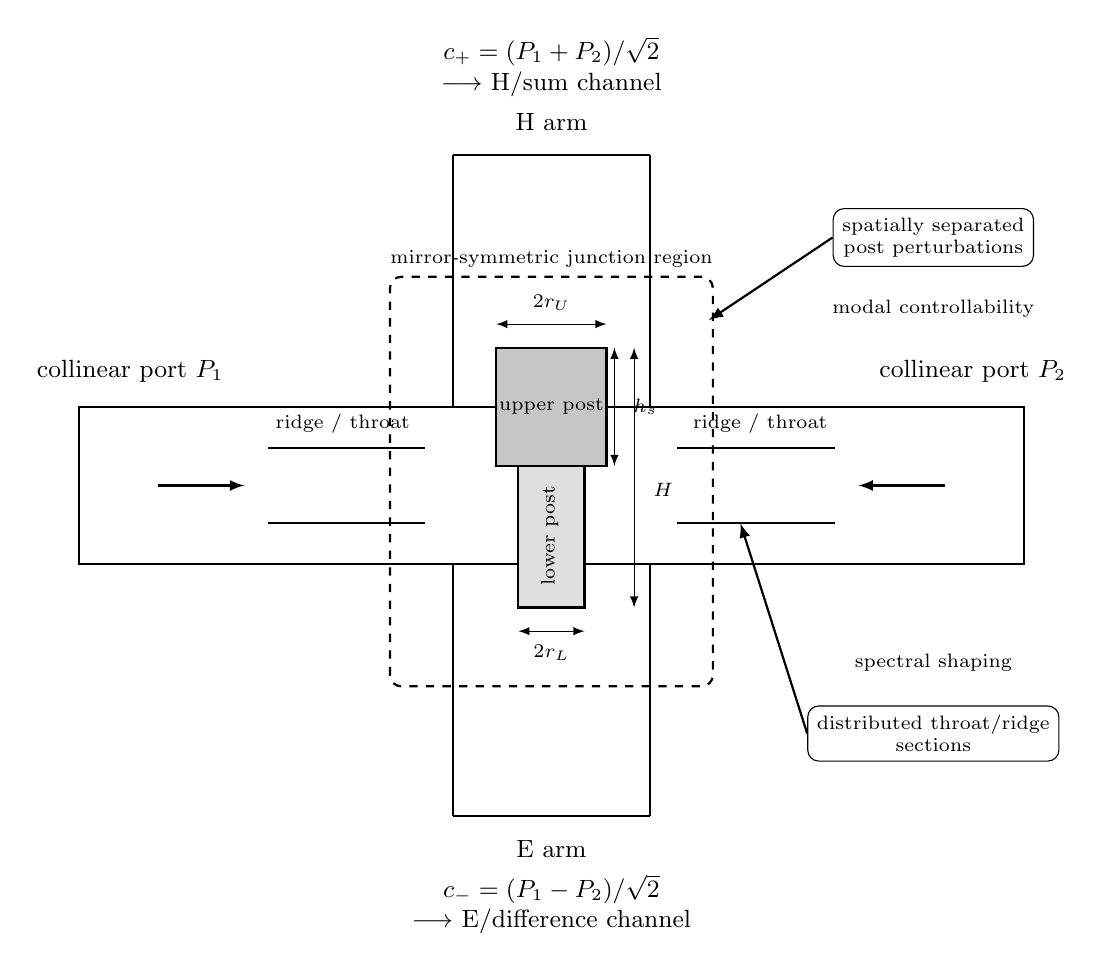
\begin{tikzpicture}[x=1cm,y=1cm,>=latex]

% Main collinear guide
\draw[thick] (-6,-1.0) rectangle (6,1.0);
\draw[thick] (-6,1.0) -- (-6,-1.0);
\draw[thick] (6,1.0) -- (6,-1.0);

% H arm
\draw[thick] (-1.25,1.0) -- (-1.25,4.2);
\draw[thick] (1.25,1.0) -- (1.25,4.2);
\draw[thick] (-1.25,4.2) -- (1.25,4.2);

% E arm
\draw[thick] (-1.25,-1.0) -- (-1.25,-4.2);
\draw[thick] (1.25,-1.0) -- (1.25,-4.2);
\draw[thick] (-1.25,-4.2) -- (1.25,-4.2);

% Central stepped post
\fill[gray!25] (-0.42,-1.55) rectangle (0.42,0.25);
\fill[gray!45] (-0.70,0.25) rectangle (0.70,1.75);
\draw[thick] (-0.42,-1.55) rectangle (0.42,0.25);
\draw[thick] (-0.70,0.25) rectangle (0.70,1.75);

% Throat / ridge hints
\draw[thick] (-3.6,0.48) -- (-1.6,0.48);
\draw[thick] (-3.6,-0.48) -- (-1.6,-0.48);
\draw[thick] (1.6,0.48) -- (3.6,0.48);
\draw[thick] (1.6,-0.48) -- (3.6,-0.48);
\node[font=\scriptsize] at (2.65,0.78) {ridge / throat};
\node[font=\scriptsize] at (-2.65,0.78) {ridge / throat};

% Physical ports
\node[font=\small] at (-5.35,1.45) {collinear port $P_1$};
\node[font=\small] at (5.35,1.45) {collinear port $P_2$};
\node[font=\small] at (0,4.62) {H arm};
\node[font=\small] at (0,-4.62) {E arm};

% Modal arrows / labels
\draw[->,thick] (-5.0,0) -- (-3.9,0);
\draw[->,thick] (5.0,0) -- (3.9,0);
\node[font=\small,align=center] at (0,5.32)
{$c_+=(P_1+P_2)/\sqrt2$\\$\longrightarrow$ H/sum channel};
\node[font=\small,align=center] at (0,-5.32)
{$c_-=(P_1-P_2)/\sqrt2$\\$\longrightarrow$ E/difference channel};

% Geometry annotations
\draw[<->] (0.80,0.25) -- (0.80,1.75);
\node[font=\scriptsize,anchor=west] at (0.92,1.0) {$h_s$};

\draw[<->] (1.05,-1.55) -- (1.05,1.75);
\node[font=\scriptsize,anchor=west] at (1.17,-0.05) {$H$};

\draw[<->] (-0.42,-1.85) -- (0.42,-1.85);
\node[font=\scriptsize] at (0,-2.12) {$2r_L$};

\draw[<->] (-0.70,2.05) -- (0.70,2.05);
\node[font=\scriptsize] at (0,2.32) {$2r_U$};

% Region labels
\node[font=\scriptsize,rotate=90] at (-0.02,-0.64) {lower post};
\node[font=\scriptsize] at (0,1.00) {upper post};

% Parity-protection callout
\draw[rounded corners,thick,dashed] (-2.05,-2.55) rectangle (2.05,2.65);
\node[font=\scriptsize,align=center] at (0,2.88)
{mirror-symmetric junction region};

% Concept arrows to interpretation
\node[draw,rounded corners,align=center,font=\scriptsize] (modal) at (4.85,3.15)
{spatially separated\\post perturbations};
\node[draw,rounded corners,align=center,font=\scriptsize] (spectral) at (4.85,-3.15)
{distributed throat/ridge\\sections};

\draw[->,thick] (modal.west) -- (2.0,2.1);
\draw[->,thick] (spectral.west) -- (2.4,-0.48);

\node[font=\scriptsize,align=center] at (4.85,2.25)
{modal controllability};
\node[font=\scriptsize,align=center] at (4.85,-2.25)
{spectral shaping};

\end{tikzpicture}
\caption{Reader-oriented schematic of the broadband Magic-T cell and the two-layer design interpretation. Mirror symmetry separates the collinear excitation into the even state $c_+$, which couples to the H/sum arm, and the odd state $c_-$, which couples to the E/difference arm. The stepped post introduces spatially separated lower and upper perturbation regions parameterized by $r_L$, $r_U$, $h_s$, and total height $H$; these provide local modal-control directions. The distributed throat/ridge sections primarily shape the frequency dependence of the two allowed modal reflections. The drawing is schematic and is intended to clarify the control architecture rather than reproduce manufacturing dimensions.}
\label{fig:geometry-schematic}
\end{figure*}
